\documentclass[10pt]{report}

\usepackage{talks}
\newcommand{\expect}[1]{\mathbb{E}\!\left[ #1 \right]}
\newcommand{\reals}{\mathbb{R}}
\newcommand{\draw}[2]{#1^{(#2)}}
\usepackage{mathpazo}
\usepackage{sourcecodepro}
\usepackage{tikz}
    \usetikzlibrary{positioning, shapes, arrows.meta}

\newcommand{\ddfrac}[2]{\frac{\strut \displaystyle #1}{\strut \displaystyle #2}}
    
\begin{document}

\sf \mbox{}
\\[12pt]
\spc{\LARGE\bfseries \color{MidnightBlue}{50 years of word embeddings}}
\\[40pt]
\noindent 
\spc{\large\bfseries \color{MidnightBlue}{Bob Carpenter}}
\\[2pt]
\spc{\small Center for Computational Mathematics}
\\[-1pt]
\spc{\small Flatiron Institute}
\\[2pt]
\spc{\footnotesize \url{bcarpenter@flatironinstitute.org}}
\vfill 
\noindent 
\spc{\footnotesize December 2023 \qquad CCM Transformer Reading Group}
\hfill

\includegraphics[width=1.25in]{img/flatiron-logo.png}


\sld{What's a word embedding}
\begin{itemize}
\item Let $W$ be the \myemph{number of distinct words}.
\item Let $P$ be the \myemph{embedding dimension}.
\item Let   $[W] = \{ 0, \ldots, W - 1 \}$ be the set of words.
\item A \myemph{word embedding} is a function $f \, \textrm{:} \, [W] \rightarrow \mathbb{R}^P$.
\vfill
\item Assuming \myemph{finitely many words} is problematic
  \begin{subitemize}
  \item what's a word? (e.g., Chinese)
  \item productive morphology? (e.g., Turkish, German, or even English)
  \end{subitemize}
\end{itemize}

\sld{Document-based word embeddings}
\begin{subitemize}
\item \textit{You shall know a word by the company it keeps.} (Firth 1957) 
\item Rows: \myemph{word embeddings}, Columns: \myemph{document embeddings}
\end{subitemize}
\begin{center}
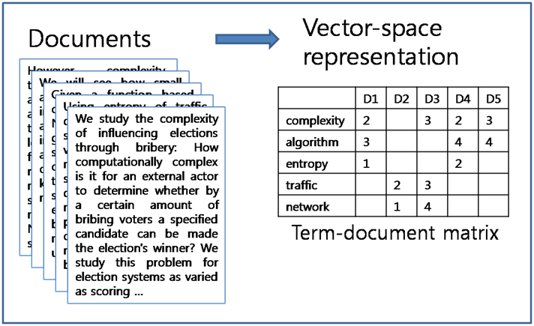
\includegraphics[width=0.55\textwidth]{img/term-doc-matrix.jpeg}
\end{center}
\vspace*{-4pt}
\spc {\footnotesize From: \tiny \texttt{https://www.quora.com/What-is-a-term-document-matrix}}

\sld{Document retrieval (cont.)}
\begin{itemize}
\item A \myemph{search query} $q$ is embedded like a document (word frequency).
\item Score document $d$ for query $q$ using \myemph{cosine}
  between embedding vectors $g(d)$ and $g(q)$
  $$
  \textrm{dist}(d, q) = g(d)^{\top} \cdot g(q)
  $$
\item Smaller angle is ``closer.''
\end{itemize}
\vfill
\spc  {\small (Salton 1968)}

\sld{TF-IDF: Inverse document frequency}
\begin{itemize}
\item Let the tinkering begin!
  \vspace*{12pt}
\item The \myemph{term frequency} of a word is just its document
  embedding as word counts.
\item Intuition is to \myemph{downweight common words}.
\item Divide word frequency by document frequency
  \begin{subitemize}
  \item multiply by \myemph{inverse document frequency} (IDF)
  \end{subitemize}
\item Resulting document and word embeddings called \myemph{TF-IDF}.
\end{itemize}
\vfill
\spc {\small (Sp\"arck Jones 1972)}

\sld{Latent semantic analysis (LSA)}
\begin{itemize}
\item Take $W \times D$ TF-IDF matrix $X$ and singular value decompose,
  $$
  X = U \cdot \textrm{diagMat}(S) \cdot V^{\top},
  $$
  with $U$ and $V$ orthonormal, $S$ non-negative descending
\item Restrict to rank $K < \textrm{min}(D, W)$ by taking
  $X \approx U_{1\textrm{:}W,1\textrm{:}K} \cdot \textrm{diagMat}(S_{1\textrm{:}K}) \cdot V_{1\textrm{:}D,
    1\textrm{:}K}^{\top}$
\item Minimizes square error at rank $K$
\item Use $U_{w,1\textrm{:}K}$ as document embedding and $V_{d,1\textrm{:}K}$ as
  document embedding (both embedded in $\mathbb{R}^K$).
\item Embed queries by \myemph{sum of word embeddings} and compare with cosine. 
\end{itemize}
\vfill
\spc {\small (Dumais, Furnas, Landauer, Deerwester 1988)}

\sld{Word embeddings for language modeling}
\begin{itemize}
\item Embed words.
\item Apply \myemph{hierarchical clustering} to the word embeddings.
\item Use classes from clusters to smooth $n$-gram language models.
\item This found all sorts of uses, including as covariate extractors
  for classification.
\end{itemize}
\vfill
\spc {\small (Brown, de Souza, Mercer, Della Pietra, Lai, 1992)}


\sld{Pure text embeddings and skip-grams}
\begin{itemize}
\item Instead of word by documents, just use a corpus of text.
\item Model a word by frequencies of \myemph{words appearing around it}
  (i.e., the ``company it keeps'')
\item Allow skipping, dubbed a \myemph{skip-gram} (vs. contiguous
  \myemph{n-gram}).
\item Use like every other embedding.
  \vfill
  \spc {\small (Rosenfeld 1994), etc.}
  \\
  \spc {\small (Guthrie, Allison, Liu, Guthrie, Wilks 2006) \myemph{survey})}
\end{itemize}

\sld{Word embeddings as covariates}
\begin{itemize}
\item People used \myemph{word embeddings as predictors} in
  classifiers.
\item Map a query to the sum of the low-rank embeddings of its words.
\item For example, we used them in \myemph{logistic regression} for call routing
  (target modeled as sum of training queries)
\item We also used them to \myemph{disambiguate ambiguous queries}
  (e.g., difference of destination embedding vectors minus query)
  \\
\vfill
\spc {\small Carpenter and Chu-Carroll, 1999 (paper), 2001 (patent)}
\end{itemize}

\sld{Latent Dirichlet Allocation (LDA)}
\begin{itemize}
\item LDA is a Bayesian version of the LSA factor model
  \begin{subitemize}
  \item i.e., a \myemph{mixed-membership} mixture model
  \end{subitemize}
\item Documents modeled as an distribution of topics: $\theta_d \sim \textrm{Dirichlet}(\alpha)$
\item Words independently drawn from topics:\\ $z_{d,n} \sim
  \textrm{Categorical}(\theta_d)$ \qquad \quad $w_{d,n} \sim \textrm{Categorical}(\phi_{z_{d,n}})$.
\item Induces word-word similarity vectors by expected co-occurrence
  in documents (vs. adjacency or near adjacency in skip-grams).
\item Document embeddings as topic mixture used as covariates
  (features) for an SVM classifier.
\end{itemize}
\vfill
\spc {\small (Blei, Ng, Jordan 2003)}

\sld{What is Word2Vec?}
\begin{itemize}
\item Train \myemph{discriminative word classifier} based on context
  \begin{subitemize}
  \item 4 past and 4 future tokens and \myemph{$n$-grams} in a
    \myemph{bag of words} (no order)
  \item skip-grams (more distant words in past and future context)
  \end{subitemize}
\item Architecture is \myemph{not autoregressive}, but generation not goal.
\item Feedforward and recursive neural net architectures.
\item Tested with \myemph{word similarity} (cf. LSA): skip-gram +
  recursive net win.
\item \myemph{Open-source} software. 
\end{itemize}
\vfill 
\spc {\small (Mikolov, Sutskever, Chen, Corrado, Dean 2013)}

\sld{23 Skidoo (i.e., nothing to see, move along)}
\begin{itemize}
\item Word2Vec \myemph{Superseded} by jointly optimized transformer embeddings 
\end{itemize}
\begin{center}
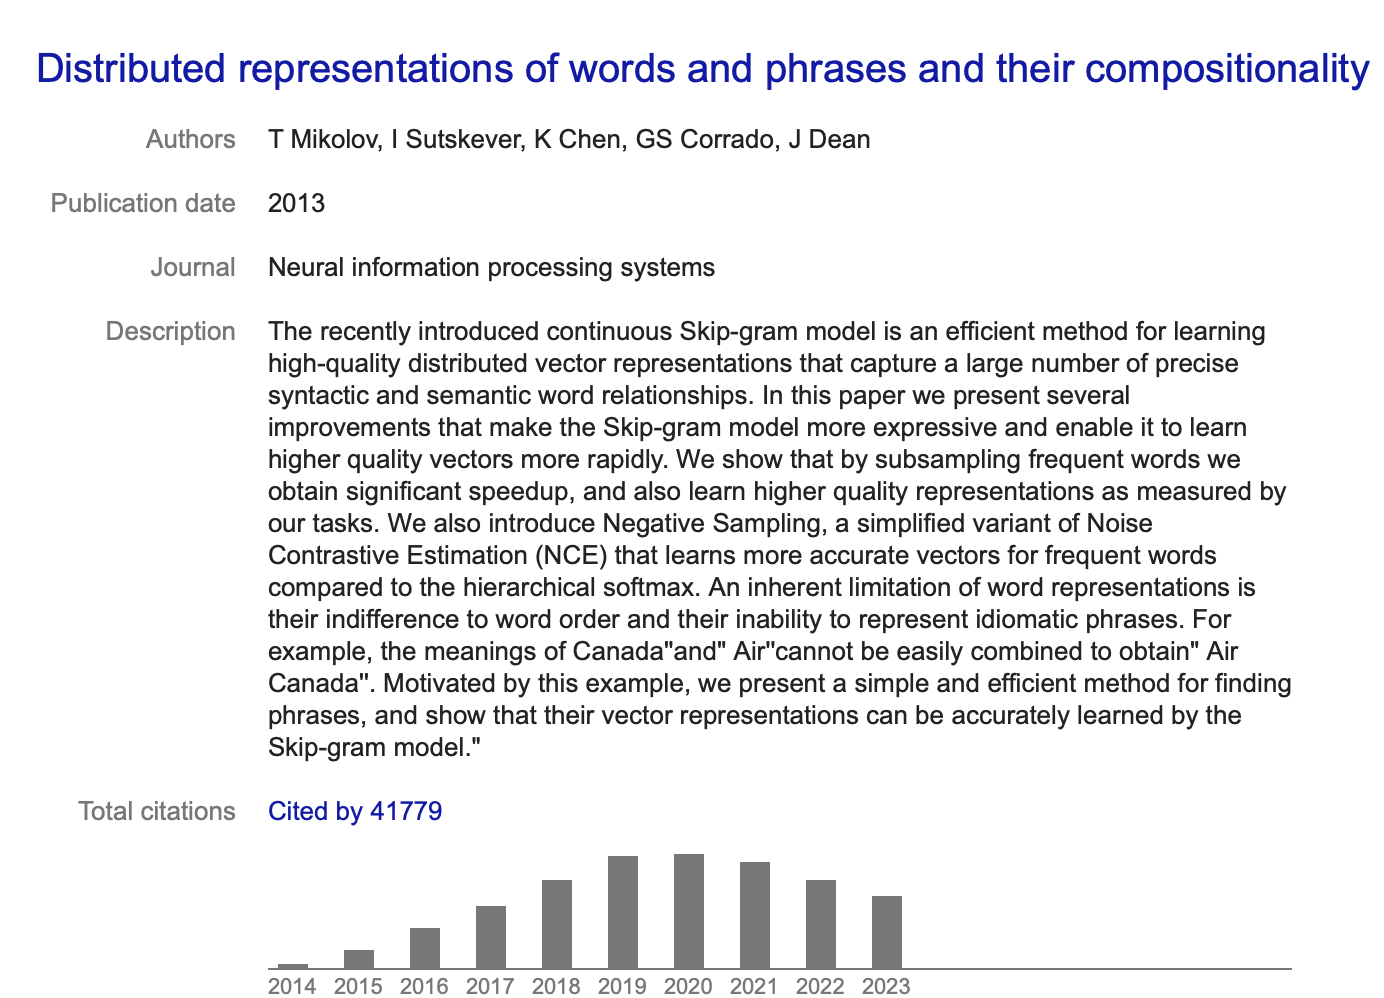
\includegraphics[width=2.5in]{img/word2vec.png}
\end{center}

\end{document}
